\documentclass[12pt,a4paper]{scrartcl} 
\usepackage[utf8]{inputenc}
\usepackage[english,russian]{babel}
\usepackage{indentfirst}
\usepackage{misccorr}
\usepackage{graphicx}
\usepackage{indentfirst}
\usepackage{amsmath}
\begin{document}
 \begin{titlepage}
  \begin{center}
   \large
   МИНИСТЕРСТВО НАУКИ И ВЫСШЕГО ОБРАЗОВАНИЯ РОССИЙСКОЙ ФЕДЕРАЦИИ
   
   Федеральное государственное бюджетное образовательное учреждение высшего образования
   
   \textbf{АДЫГЕЙСКИЙ ГОСУДАРСТВЕННЫЙ УНИВЕРСИТЕТ}
   \vspace{0.25cm}
   
   Инженерно-физический факультет
   
   Кафедра автоматизированных систем обработки информации и управления
   \vfill

   \vfill
   
   \textsc{Отчет по практике}\\[5mm]
   
   {\LARGE \textit{Кратчайшие пути на графе}}
   \bigskip
   
   2 курс, группа 2ИВТ1-2
  \end{center}
  \vfill
  
  \newlength{\ML}
  \settowidth{\ML}{«\underline{\hspace{0.7cm}}» \underline{\hspace{2cm}}}
  \hfill\begin{minipage}{0.5\textwidth}
   Выполнила:\\
   \underline{\hspace{\ML}} Т.\,И.~Андрощук\\
   «\underline{\hspace{0.7cm}}» \underline{\hspace{2cm}} 2024 г.
  \end{minipage}%
  \bigskip
  
  \hfill\begin{minipage}{0.5\textwidth}
   Руководитель:\\
   \underline{\hspace{\ML}} С.\,В.~Теплоухов\\
   «\underline{\hspace{0.7cm}}» \underline{\hspace{2cm}} 2024 г.
  \end{minipage}%
  \vfill
  
  \begin{center}
   Майкоп, 2024 г.
  \end{center}
 \end{titlepage}
 

\section{Введение}
\label{sec:intro}


\subsection{Формулировка цели}
Целью данной работы является написание программы для нахождение кратчайшего пути на графе.

\section{Ход работы}
\label{sec:exp}

\subsection{Код приложения}
\label{sec:exp:code}
\begin{verbatim}
#include<iostream>
using namespace std;
int main()
{
	setlocale(LC_ALL, "Russian");
	int a[6][6]; 
	int d[6]; 
	int v[6]; 
	int temp, minindex, min;
	int begin_index = 0;
	for (int i = 0; i < 6; i++) { 
		a[i][i] = 0;
		for (int j = i + 1; j < 6; j++) {
			cout << "Введите расстояние " << i + 1 << " - " << j + 1 << ": ";
			cin >> temp;
			a[i][j] = temp;
			a[j][i] = temp;
		}
	}
	for (int i = 0; i < 6; i++) {
		for (int j = 0; j < 6; j++) {
			cout << " " << a[i][j];
		}
		cout << endl;
	}
	for (int i = 0; i < 6; i++) { 
		d[i] = 10000;
		v[i] = 1;
	}
	d[begin_index] = 0;
	do {
		minindex = 10000;
		min = 10000;
		for (int i = 0; i < 6; i++) { 
			if ((v[i] == 1) && (d[i] < min)) { 
				min = d[i];
				minindex = i;
			}
		}
		if (minindex != 10000) {
			for (int i = 0; i < 6; i++) {
				if (a[minindex][i] > 0) {
					temp = min + a[minindex][i];
					if (temp < d[i]) {
						d[i] = temp;
					}
				}
			}
			v[minindex] = 0;
		}
	} while (minindex < 10000);
	cout << endl << "Кратчайшие расстояния до вершин:" << endl;
	for (int i = 0; i < 6; i++) {
		cout << " " << d[i];
	}
	
	int ver[6]; 
	int end = 4; 
	ver[0] = end + 1; 
	int k = 1; 
	int weight = d[end]; 
	while (end != begin_index) { 
		for (int i = 0; i < 6; i++) {
			if (a[i][end] != 0) { 
				int temp = weight - a[i][end]; 
					if (temp == d[i]) {  
							weight = temp; 
						end = i; 
						ver[k] = i + 1;
						k++;
					}
			}
		}
	}
	cout << endl << "Вывод кратчайшего пути" << endl;
	for (int i = k - 1; i >= 0; i--) {
		cout << " " << ver[i];
	}
}
\end{verbatim}


\section{Скриншоты программы}

\label{sec:picexample}
\begin{figure}[h]
	\begin{center}
    \begin{minipage}{0.39\linewidth}
	  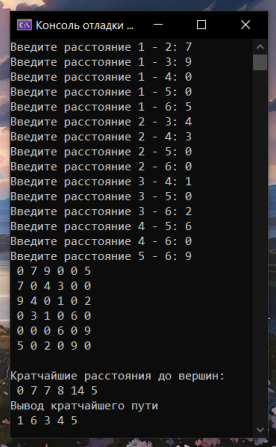
\includegraphics[width=1\textwidth]{Решение.PNG}
	  \caption{Решение}\label{fig:par}
    \end{minipage}
    \end{center}
\end{figure}



\begin{thebibliography}{9}
\bibitem{Knuth-2003}Кнут Д.Э. Всё про \TeX. \newblock --- Москва: Изд. Вильямс, 2003 г. 550~с.
\bibitem{Lvovsky-2003}Львовский С.М. Набор и верстка в системе \LaTeX{}. \newblock --- 3-е издание, исправленное и дополненное, 2003 г.
\bibitem{Voroncov-2005}Воронцов К.В. \LaTeX{} в примерах. 2005 г.
\end{thebibliography}

\end{document}
